\documentclass[]{article}
\usepackage[margin=2cm]{geometry}

%opening
\title{Exercises Set: Constrained Optimization\\ \large Solutions}
\author{DSBA Mathematics Refresher 2026}
\date{}

\usepackage{amsmath}
\usepackage{amsfonts}
\usepackage{amsthm}
\usepackage{amssymb}
\usepackage{mathrsfs}
\usepackage{stmaryrd}
\usepackage{tikz}
\usepackage{tikz}

\newcommand{\Q}{\mathbb{Q}}
\newcommand{\N}{\mathbb{N}}
\newcommand{\Z}{\mathbb{Z}}
\newcommand{\R}{\mathbb{R}}
\newcommand{\Primes}{\mathbb{P}}
\newcommand{\st}{\text{ s.t. }}
\newcommand{\txtand}{\text{ and }}
\newcommand{\txtor}{\text{ or }}
\newcommand{\lxor}{\veebar}
\newcommand{\vecx}{ \vec{\mathbf{x}} }
\newcommand{\vecxk}{ \vec{\mathbf{x_k}} }
\newcommand{\vecw}{ \vec{\mathbf{w}} }



\begin{document}

	\maketitle

	\section{Lagrangian multiplier technique}

	\subsection{Unconstrained optimization}

	$f(x,y) = 2x^2 - 12x + 4y^2 + 8y + 20$.

	We set both partial derivatives to zero:
	$$
	\frac{\partial f}{\partial x} = 4x - 12 = 0
	\qquad \text{and} \qquad
	\frac{\partial f}{\partial y} = 8y + 8 = 0
	$$
	which gives $x^* = 3$ and $y^* = -1$, with
	$$
	f(3,-1) = 18 - 36 + 4 - 8 + 20 = -2
	$$

	This point is indeed a \textit{minimum} (and not a maximum or a saddle point), as one sees by completing the squares:
	$$
	f(x,y) = 2(x-3)^2 + 4(y+1)^2 - 2
	$$
	Both squares are non-negative, so $f(x,y) \geq -2$ for every $(x,y)$, with equality only at $(3,-1)$.
	We will re-use this form below.

	\subsection{(Equality) Constrained optimization}

	Same $f$, with the constraint $3x + 5y = 2$.

	We solve the constraint for $y$:
	$$
	y = \frac{2 - 3x}{5}
	$$
	and substitute it into $f$, which becomes a function of $x$ alone:
	$$
	f\left(x, \frac{2-3x}{5}\right)
	= 2x^2 - 12x + 4\left(\frac{2-3x}{5}\right)^2 + 8\left(\frac{2-3x}{5}\right) + 20
	= \frac{86x^2 - 468x + 596}{25}
	$$
	Setting the derivative to zero:
	$$
	\frac{172x - 468}{25} = 0
	\qquad \Longrightarrow \qquad
	x^* = \frac{468}{172} = \frac{117}{43} \approx 2.721
	$$
	and then
	$$
	y^* = \frac{2 - 3 \cdot \frac{117}{43}}{5} = \frac{\frac{86 - 351}{43}}{5} = -\frac{53}{43} \approx -1.233
	$$
	Using the completed-square form, the minimum value is
	$$
	f(x^*,y^*) = 2\left(-\frac{12}{43}\right)^2 + 4\left(-\frac{10}{43}\right)^2 - 2 = \frac{688}{1849} - 2 = \frac{16}{43} - 2 = -\frac{70}{43} \approx -1.628
	$$
	As expected, this is \textit{larger} than the unconstrained minimum $-2$: adding a constraint can only make the minimum worse (or leave it unchanged).

	\subsection{Lagrange multiplier (*)}

	Same problem, with $\mathcal{L}(x,y,\lambda) = f(x,y) - \lambda(3x + 5y - 2)$.

	The three partial derivatives give:
	$$
	\frac{\partial \mathcal{L}}{\partial x} = 4x - 12 - 3\lambda = 0,
	\qquad
	\frac{\partial \mathcal{L}}{\partial y} = 8y + 8 - 5\lambda = 0,
	\qquad
	\frac{\partial \mathcal{L}}{\partial \lambda} = -(3x + 5y - 2) = 0
	$$
	The first two give
	$$
	x = \frac{3\lambda + 12}{4}
	\qquad \text{and} \qquad
	y = \frac{5\lambda - 8}{8}
	$$
	Substituting into the third (the constraint), and multiplying by $8$:
	$$
	6(3\lambda + 12) + 5(5\lambda - 8) = 16
	\quad \Longrightarrow \quad
	43\lambda + 32 = 16
	\quad \Longrightarrow \quad
	\lambda = -\frac{16}{43}
	$$
	and therefore
	$$
	x^* = \frac{117}{43}, \qquad y^* = -\frac{53}{43}
	$$
	which is exactly the answer found by substitution. \checkmark

	\begin{center}
		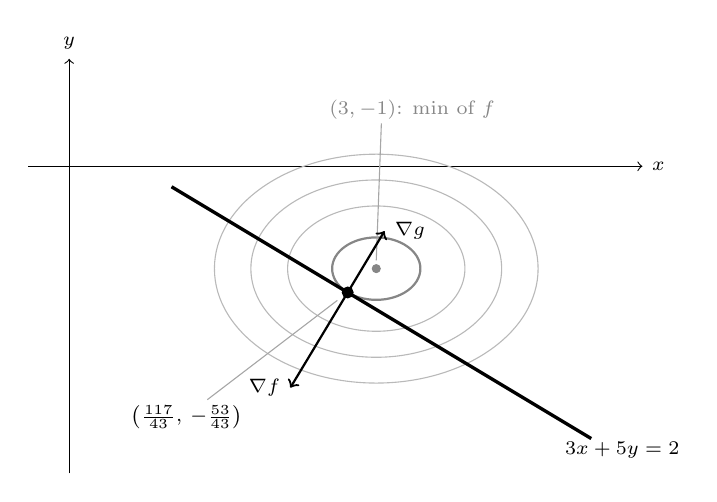
\begin{tikzpicture}[scale=1.3]
			\draw[->] (-0.4,0) -- (5.6,0) node[right] {\scriptsize $x$};
			\draw[->] (0,-3.0) -- (0,1.05) node[above] {\scriptsize $y$};
			% level ellipses of f, centred at the unconstrained minimum (3,-1)
			\draw[gray!55] (3,-1) ellipse (1.581 and 1.118);
			\draw[gray!55] (3,-1) ellipse (1.225 and 0.866);
			\draw[gray!55] (3,-1) ellipse (0.866 and 0.612);
			\draw[thick,gray!95] (3,-1) ellipse (0.431 and 0.305);
			\filldraw[gray!95] (3,-1) circle (1.1pt);
			\node[gray!95] at (3.35,0.55) {\scriptsize $(3,-1)$: min of $f$};
			\draw[gray!70] (3.05,0.42) -- (3.0,-0.92);
			% the constraint
			\draw[very thick] (1,-0.2) -- (5.1,-2.66);
			\node[below right] at (4.75,-2.6) {\scriptsize $3x+5y=2$};
			% the optimum
			\filldraw (2.721,-1.233) circle (1.5pt);
			\node at (1.15,-2.45) {\scriptsize $\left(\frac{117}{43},\,-\frac{53}{43}\right)$};
			\draw[gray!70] (1.35,-2.28) -- (2.62,-1.31);
			% gradients
			\draw[->,thick] (2.721,-1.233) -- ++(-0.56,-0.93) node[left] {\scriptsize $\nabla f$};
			\draw[->,thick] (2.721,-1.233) -- ++(0.36,0.60) node[right] {\scriptsize $\nabla g$};
		\end{tikzpicture}
	\end{center}
	The level curves of $f$ are ellipses centred on the unconstrained minimum $(3,-1)$.
	Walking along the line, we cross smaller and smaller ellipses until one of them merely \textit{touches} the line: that tangency point is the constrained optimum.
	At that point the two gradients are parallel (here they point in \textit{opposite} directions, which is exactly what $\lambda = -\frac{16}{43} < 0$ means).

	Note that the third equation $\frac{\partial \mathcal{L}}{\partial \lambda} = 0$ is nothing but the constraint itself: this is why the method works.

	\subsection{(Inequality) Constrained optimization}

	\paragraph{First case:} $f(x) = x^2 - 2x$, with $3x \leq 2$, i.e. $x \leq \frac{2}{3}$.

	The unconstrained minimum is at $f'(x) = 2x - 2 = 0$, i.e. $x = 1$.
	But $3 \times 1 = 3 > 2$, so this point is \textbf{not allowed}.

	On the allowed region, $f$ is decreasing (since $f'(x) = 2x - 2 < 0$ for $x < 1$), so the smallest value is reached at the right end of the interval:
	$$
	x^* = \frac{2}{3},
	\qquad
	f(x^*) = \frac{4}{9} - \frac{4}{3} = -\frac{8}{9}
	$$
	The constraint is \textbf{active}: it "pushes" the solution away from the unconstrained minimum.

	\paragraph{Second case:} $f(x) = x^2 + 2x$, with $3x \leq 2$.

	The unconstrained minimum is at $f'(x) = 2x + 2 = 0$, i.e. $x = -1$.
	This time $3 \times (-1) = -3 \leq 2$, so the point \textbf{is allowed}, and it is therefore also the solution of the constrained problem:
	$$
	x^* = -1, \qquad f(x^*) = -1
	$$
	The constraint is \textbf{inactive}: it changes nothing.

	\subsection{Lagrange multiplier (*)}

	With $g(x) = -3x + 2 \geq 0$ and the slack variable $s$, the Lagrangian is
	$$
	\mathcal{L}(x,s,\lambda) = f(x) - \lambda\left(-3x + 2 - s^2\right)
	$$
	and the partial derivatives with respect to $s$ and $\lambda$ are the same in both cases:
	$$
	\frac{\partial \mathcal{L}}{\partial s} = 2\lambda s = 0
	\qquad \text{and} \qquad
	\frac{\partial \mathcal{L}}{\partial \lambda} = 3x - 2 + s^2 = 0
	$$
	The equation $\lambda s = 0$ forces us to consider two cases: either $\lambda = 0$ (the constraint is ignored), or $s = 0$ (the constraint is an equality).

	\paragraph{First case:} $f(x) = x^2 - 2x$, so $\frac{\partial \mathcal{L}}{\partial x} = 2x - 2 + 3\lambda = 0$.
	\begin{itemize}
		\item If $\lambda = 0$: then $x = 1$, and $s^2 = 2 - 3x = -1 < 0$, which is impossible ($s^2 \geq 0$).
		This case is rejected (it is the algebraic way of saying that the unconstrained minimum is not allowed).
		\item If $s = 0$: then $3x = 2$, i.e. $x = \frac{2}{3}$, and $2\left(\frac{2}{3}\right) - 2 + 3\lambda = 0$ gives $\lambda = \frac{2}{9} \geq 0$. \checkmark
	\end{itemize}
	So $x^* = \frac{2}{3}$ with $\lambda = \frac{2}{9} > 0$, as found before. \checkmark

	\paragraph{Second case:} $f(x) = x^2 + 2x$, so $\frac{\partial \mathcal{L}}{\partial x} = 2x + 2 + 3\lambda = 0$.
	\begin{itemize}
		\item If $\lambda = 0$: then $x = -1$, and $s^2 = 2 - 3x = 5 \geq 0$. \checkmark \ This case is valid.
		\item If $s = 0$: then $x = \frac{2}{3}$, and $2\left(\frac{2}{3}\right) + 2 + 3\lambda = 0$ gives $\lambda = -\frac{10}{9} < 0$, which violates the condition $\lambda \geq 0$.
		This case is rejected.
	\end{itemize}
	So $x^* = -1$ with $\lambda = 0$, as found before. \checkmark

	\paragraph{Comparison.}
	We found $\lambda = 0$ in the second case, which is the one where the constraint did nothing.
	This is general:
	$$
	\lambda = 0 \iff \text{the constraint is inactive}
	$$
	Indeed, $\lambda$ measures how hard the constraint "pushes" on the solution (see Section 1.9): if the unconstrained minimum is already allowed, there is nothing to push, and $\lambda = 0$.
	The condition $\lambda s = 0$ (one of the two must be zero) is known as \textbf{complementary slackness}, and the requirement $\lambda \geq 0$ ensures that the constraint pushes in the right direction, with $\lambda < 0$ we would be at a \textit{maximum} along the boundary rather than a minimum.

	\subsection{Distance from a point to a line}

	$f(x,y) = x^2 + y^2$, with $2x + y = 5$.

	\paragraph{1. Geometrically.}
	$f$ is the squared distance from $(x,y)$ to the origin, so we are looking for the point of the line closest to the origin.
	That point is the foot of the perpendicular dropped from the origin onto the line.
	The vector $\begin{pmatrix} 2 \\ 1 \end{pmatrix}$ is normal to the line $2x + y = 5$, so the point we want is of the form $t\begin{pmatrix} 2 \\ 1 \end{pmatrix}$, and the constraint gives
	$$
	2(2t) + t = 5 \quad \Longrightarrow \quad 5t = 5 \quad \Longrightarrow \quad t = 1
	$$
	so the closest point is $(2,1)$, at squared distance $f(2,1) = 5$ (i.e. at distance $\sqrt{5}$).

	\paragraph{2. By substitution.}
	The constraint gives $y = 5 - 2x$, so
	$$
	f(x, 5-2x) = x^2 + (5-2x)^2 = 5x^2 - 20x + 25
	$$
	Setting the derivative to zero: $10x - 20 = 0$, so $x^* = 2$ and $y^* = 5 - 4 = 1$. \checkmark

	\paragraph{3. With a Lagrange multiplier.}
	With $\mathcal{L}(x,y,\lambda) = x^2 + y^2 - \lambda(2x + y - 5)$:
	$$
	\frac{\partial \mathcal{L}}{\partial x} = 2x - 2\lambda = 0,
	\qquad
	\frac{\partial \mathcal{L}}{\partial y} = 2y - \lambda = 0,
	\qquad
	\frac{\partial \mathcal{L}}{\partial \lambda} = -(2x + y - 5) = 0
	$$
	The first two give $x = \lambda$ and $y = \frac{\lambda}{2}$; the constraint then gives $2\lambda + \frac{\lambda}{2} = 5$, i.e. $\lambda = 2$, hence
	$$
	x^* = 2, \qquad y^* = 1
	$$
	The three methods agree. \checkmark

	Note that the solution $(2,1)$ is proportional to the normal vector $\begin{pmatrix} 2 \\ 1 \end{pmatrix}$, which is exactly what the geometric argument predicted: $\nabla f = \begin{pmatrix} 2x \\ 2y \end{pmatrix}$ must be parallel to $\nabla g = \begin{pmatrix} 2 \\ 1 \end{pmatrix}$.

	\subsection{A constraint that cannot be substituted}

	$f(x,y) = x + y$, with $x^2 + y^2 = 1$.

	\paragraph{1. What goes wrong with substitution.}
	Solving the constraint for $y$ gives
	$$
	y = \pm\sqrt{1 - x^2}
	$$
	which is not \textit{one} function but \textit{two} (the upper and the lower half of the circle), so we would have to treat two separate problems.
	Worse, $\sqrt{1-x^2}$ is not differentiable at $x = \pm 1$, and those two points would have to be checked separately.
	The substitution method still works here, but it is already unpleasant, and it becomes impossible as soon as the constraint cannot be solved explicitly.

	\paragraph{2. With a Lagrange multiplier.}
	With $\mathcal{L}(x,y,\lambda) = x + y - \lambda(x^2 + y^2 - 1)$:
	$$
	\frac{\partial \mathcal{L}}{\partial x} = 1 - 2\lambda x = 0,
	\qquad
	\frac{\partial \mathcal{L}}{\partial y} = 1 - 2\lambda y = 0,
	\qquad
	\frac{\partial \mathcal{L}}{\partial \lambda} = -(x^2 + y^2 - 1) = 0
	$$
	The first equation shows that $\lambda \neq 0$ (otherwise it would read $1 = 0$), so we can write $x = \frac{1}{2\lambda}$ and $y = \frac{1}{2\lambda}$: the first two equations give $x = y$.
	The constraint then gives $2x^2 = 1$, so
	$$
	x = y = \frac{1}{\sqrt{2}}
	\qquad \text{or} \qquad
	x = y = -\frac{1}{\sqrt{2}}
	$$

	\paragraph{3. Which is which.}
	$$
	f\left(\tfrac{1}{\sqrt{2}}, \tfrac{1}{\sqrt{2}}\right) = \frac{2}{\sqrt{2}} = \sqrt{2}
	\qquad \text{and} \qquad
	f\left(-\tfrac{1}{\sqrt{2}}, -\tfrac{1}{\sqrt{2}}\right) = -\sqrt{2}
	$$
	so the first point is the \textbf{maximum} and the second is the \textbf{minimum} of $f$ on the circle.

	Note that the method finds \textit{stationary points}: it does not tell us by itself which is a minimum and which is a maximum.
	Comparing the values of $f$ (as we just did) is the simplest way to decide.

	\paragraph{4. The level lines.}
	The level lines $x + y = c$ are parallel lines of slope $-1$.
	For $|c| < \sqrt{2}$ such a line cuts the circle; for $|c| > \sqrt{2}$ it misses it entirely.
	The two extreme cases $c = \pm\sqrt{2}$ are exactly the lines that \textbf{touch the circle without crossing it}, i.e. that are \textit{tangent} to it, at the two points found above.

	\begin{center}
		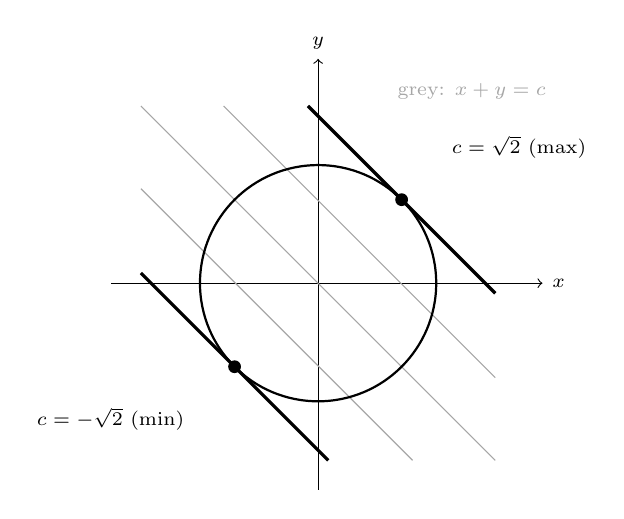
\begin{tikzpicture}[scale=1.5]
			\draw[->] (-1.75,0) -- (1.9,0) node[right] {\scriptsize $x$};
			\draw[->] (0,-1.75) -- (0,1.9) node[above] {\scriptsize $y$};
			% level lines x+y=c
			\draw[gray!70] (-1.5,1.5) -- (1.5,-1.5);
			\draw[gray!70] (-0.8,1.5) -- (1.5,-0.8);
			\draw[gray!70] (-1.5,0.8) -- (0.8,-1.5);
			\draw[very thick] (-0.086,1.5) -- (1.5,-0.086);
			\draw[very thick] (-1.5,0.086) -- (0.086,-1.5);
			\draw[thick] (0,0) circle (1);
			\filldraw (0.7071,0.7071) circle (1.4pt);
			\filldraw (-0.7071,-0.7071) circle (1.4pt);
			\node[right] at (1.05,1.15) {\scriptsize $c=\sqrt{2}$ (max)};
			\node[left] at (-1.05,-1.15) {\scriptsize $c=-\sqrt{2}$ (min)};
			\node[gray!70] at (1.3,1.62) {\scriptsize grey: $x+y=c$};
		\end{tikzpicture}
	\end{center}
	The grey lines cut the circle in two points each; the two thick ones only \textit{touch} it.
	Those are the extreme values of $c$ for which the line still meets the circle at all (beyond them, $f$ simply cannot be reached on the constraint).

	This is the geometric content of the method: at the optimum, the level line of $f$ is tangent to the constraint, so the two gradients (which are perpendicular to their respective curves) are parallel:
	$$
	\nabla f = \lambda \nabla g
	$$
	If they were not parallel, we could still slide along the constraint in the direction of decreasing $f$, and we would not be at an optimum.

	\subsection{Several constraints}

	$f(x,y,z) = x^2 + y^2 + z^2$, with $x + y + z = 6$ and $x - y = 2$.

	With $\mathcal{L}(x,y,z,\lambda,\mu) = f(x,y,z) - \lambda(x + y + z - 6) - \mu(x - y - 2)$, the derivatives with respect to $x$, $y$ and $z$ give:
	$$
	2x - \lambda - \mu = 0,
	\qquad
	2y - \lambda + \mu = 0,
	\qquad
	2z - \lambda = 0
	$$
	Adding the first two: $2(x+y) = 2\lambda$, so $x + y = \lambda$; and the third gives $z = \frac{\lambda}{2}$.
	The first constraint then reads
	$$
	\lambda + \frac{\lambda}{2} = 6
	\qquad \Longrightarrow \qquad
	\lambda = 4
	$$
	so $x + y = 4$ and $z = 2$.
	Combined with the second constraint $x - y = 2$, we get
	$$
	x^* = 3, \qquad y^* = 1, \qquad z^* = 2
	$$
	and finally $\mu = 2x - \lambda = 6 - 4 = 2$.

	The minimum value is
	$$
	f(3,1,2) = 9 + 1 + 4 = 14
	$$

	\textit{Check:} $3 + 1 + 2 = 6$ \checkmark \ and $3 - 1 = 2$. \checkmark

	Geometrically, the two constraints define a \textit{line} in $\R^3$ (the intersection of two planes), and we have found the point of that line closest to the origin, at distance $\sqrt{14}$.

	\subsection{Interpreting $\lambda$: the shadow price}

	\paragraph{1. The optimum.}
	With $\mathcal{L}(x,y,\lambda) = xy - \lambda(2x + 3y - 12)$:
	$$
	\frac{\partial \mathcal{L}}{\partial x} = y - 2\lambda = 0,
	\qquad
	\frac{\partial \mathcal{L}}{\partial y} = x - 3\lambda = 0,
	\qquad
	\frac{\partial \mathcal{L}}{\partial \lambda} = -(2x + 3y - 12) = 0
	$$
	so $y = 2\lambda$ and $x = 3\lambda$.
	The constraint gives
	$$
	2(3\lambda) + 3(2\lambda) = 12\lambda = 12
	\qquad \Longrightarrow \qquad
	\lambda = 1
	$$
	hence
	$$
	x^* = 3, \qquad y^* = 2, \qquad U(x^*,y^*) = 6
	$$
	\textit{Check:} $2 \times 3 + 3 \times 2 = 12$. \checkmark

	\paragraph{2. With a general budget $B$.}
	The two first equations are unchanged, so we still have $x = 3\lambda$ and $y = 2\lambda$; only the constraint changes:
	$$
	12\lambda = B
	\qquad \Longrightarrow \qquad
	\lambda = \frac{B}{12},
	\qquad
	x^* = \frac{B}{4},
	\qquad
	y^* = \frac{B}{6}
	$$
	and therefore
	$$
	U^*(B) = x^* y^* = \frac{B}{4} \cdot \frac{B}{6} = \frac{B^2}{24}
	$$
	\textit{Check:} for $B = 12$ we get $U^* = \frac{144}{24} = 6$. \checkmark

	\paragraph{3. The derivative.}
	$$
	\frac{dU^*}{dB} = \frac{2B}{24} = \frac{B}{12}
	\qquad \text{so at } B = 12: \qquad
	\frac{dU^*}{dB} = 1 = \lambda \ \checkmark
	$$
	The multiplier is exactly the rate at which the optimal utility improves when the budget is increased: one extra unit of budget buys (approximately) one extra unit of utility.
	This is why $\lambda$ is called the \textbf{shadow price} of the constraint, it is the most the company should be willing to pay for one extra unit of budget.

	\subsection{Inequality constraints in two dimensions}

	$f(x,y) = (x-3)^2 + (y-2)^2$ is the squared distance from $(x,y)$ to the point $(3,2)$.

	\paragraph{1. Unconstrained minimum.}
	The distance to $(3,2)$ is smallest at $(3,2)$ itself:
	$$
	x^* = 3, \qquad y^* = 2, \qquad f(x^*,y^*) = 0
	$$

	\paragraph{2. With $x + y \leq 6$.}
	We check the unconstrained minimum: $3 + 2 = 5 \leq 6$. \checkmark
	It is allowed, so it is still the solution:
	$$
	(x^*,y^*) = (3,2), \qquad f = 0
	$$
	The constraint is \textbf{inactive}.

	\paragraph{3. With $x + y \leq 4$.}
	This time $3 + 2 = 5 > 4$, so the unconstrained minimum is \textbf{not} allowed.
	The solution must therefore lie on the boundary line $x + y = 4$, and we are back to the problem of Section 1.6: find the point of that line closest to $(3,2)$.

	That point is obtained by moving from $(3,2)$ perpendicularly to the line, i.e. along the normal direction $\begin{pmatrix} 1 \\ 1 \end{pmatrix}$:
	$$
	(3,2) + t(1,1) \in \text{line}
	\quad \Longleftrightarrow \quad
	(3+t) + (2+t) = 4
	\quad \Longleftrightarrow \quad
	t = -\frac{1}{2}
	$$
	so
	$$
	(x^*,y^*) = \left(\frac{5}{2}, \frac{3}{2}\right),
	\qquad
	f(x^*,y^*) = \left(-\frac{1}{2}\right)^2 + \left(-\frac{1}{2}\right)^2 = \frac{1}{2}
	$$

	\paragraph{4. With a Lagrange multiplier and a slack variable.}
	With $\mathcal{L}(x,y,s,\lambda) = f(x,y) - \lambda(4 - x - y - s^2)$:
	$$
	\frac{\partial \mathcal{L}}{\partial x} = 2(x-3) + \lambda = 0,
	\qquad
	\frac{\partial \mathcal{L}}{\partial y} = 2(y-2) + \lambda = 0,
	$$
	$$
	\frac{\partial \mathcal{L}}{\partial s} = 2\lambda s = 0,
	\qquad
	\frac{\partial \mathcal{L}}{\partial \lambda} = -(4 - x - y - s^2) = 0
	$$
	\begin{itemize}
		\item If $\lambda = 0$: the first two equations give $(x,y) = (3,2)$, and the last one gives $s^2 = 4 - 5 = -1 < 0$, which is impossible.
		Case rejected.
		\item If $s = 0$: the constraint becomes $x + y = 4$.
		The first two equations give $2(x-3) = 2(y-2) = -\lambda$, hence $x - 3 = y - 2$, i.e. $x = y + 1$.
		Together with $x + y = 4$: $2y + 1 = 4$, so $y = \frac{3}{2}$ and $x = \frac{5}{2}$.
		Then $\lambda = -2\left(\frac{5}{2} - 3\right) = 1 \geq 0$. \checkmark
	\end{itemize}
	We recover $(x^*,y^*) = \left(\frac{5}{2}, \frac{3}{2}\right)$. \checkmark

	\begin{center}
		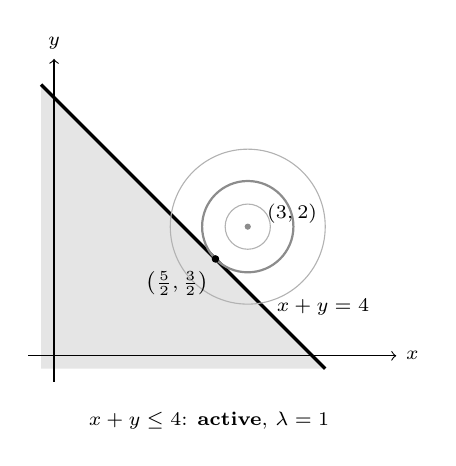
\begin{tikzpicture}[scale=0.82]
			\fill[gray!20] (-0.2,-0.2) -- (4.2,-0.2) -- (-0.2,4.2) -- cycle;
			\draw[->] (-0.4,0) -- (5.3,0) node[right] {\scriptsize $x$};
			\draw[->] (0,-0.4) -- (0,4.6) node[above] {\scriptsize $y$};
			\draw[very thick] (-0.2,4.2) -- (4.2,-0.2);
			\node[right] at (3.3,0.75) {\scriptsize $x+y=4$};
			\draw[gray!60] (3,2) circle (1.2);
			\draw[thick,gray!90] (3,2) circle (0.7071);
			\draw[gray!60] (3,2) circle (0.35);
			\filldraw[gray!90] (3,2) circle (1.1pt);
			\node[right] at (3.15,2.2) {\scriptsize $(3,2)$};
			\filldraw (2.5,1.5) circle (1.4pt);
			\node[below left] at (2.55,1.45) {\scriptsize $\left(\frac{5}{2},\frac{3}{2}\right)$};
			\node at (2.4,-1.0) {\scriptsize $x+y\leq 4$: \textbf{active}, $\lambda=1$};
		\end{tikzpicture}
		\hspace{6mm}
		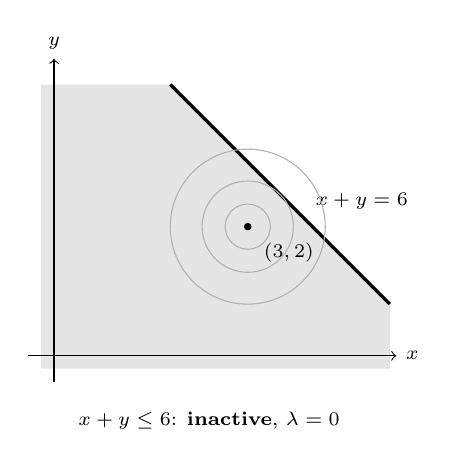
\begin{tikzpicture}[scale=0.82]
			\fill[gray!20] (-0.2,-0.2) -- (5.2,-0.2) -- (5.2,0.8) -- (1.8,4.2) -- (-0.2,4.2) -- cycle;
			\draw[->] (-0.4,0) -- (5.3,0) node[right] {\scriptsize $x$};
			\draw[->] (0,-0.4) -- (0,4.6) node[above] {\scriptsize $y$};
			\draw[very thick] (1.8,4.2) -- (5.2,0.8);
			\node[right] at (3.9,2.4) {\scriptsize $x+y=6$};
			\draw[gray!60] (3,2) circle (1.2);
			\draw[gray!60] (3,2) circle (0.7071);
			\draw[gray!60] (3,2) circle (0.35);
			\filldraw (3,2) circle (1.4pt);
			\node[below right] at (3.1,1.9) {\scriptsize $(3,2)$};
			\node at (2.4,-1.0) {\scriptsize $x+y\leq 6$: \textbf{inactive}, $\lambda=0$};
		\end{tikzpicture}
	\end{center}
	The shaded half-plane is the allowed region and the circles are the level curves of $f$ (distance to $(3,2)$).
	On the left the centre is outside the allowed region, so the best we can do is the point where a circle first touches the boundary.
	On the right the centre is already allowed, and the constraint does nothing at all.

	\paragraph{5. The value of $\lambda$.}
	In question 2 we had $\lambda = 0$, and in question 3 (and 4) we had $\lambda = 1 > 0$.

	As in Section 1.5, $\lambda = 0$ means the constraint is inactive: it could be removed without changing the answer.
	A strictly positive $\lambda$ means the constraint is active, and its value measures how much the optimum degrades as the constraint is tightened (relaxing $x + y \leq 4$ to $x + y \leq 4 + \varepsilon$ would decrease the minimum by approximately $\varepsilon$).

	\subsection{Towards Principal Component Analysis}

	$f(x,y) = 3x^2 + 2xy + 3y^2$, with $x^2 + y^2 = 1$.

	\paragraph{1. The stationarity equations.}
	With $\mathcal{L}(x,y,\lambda) = 3x^2 + 2xy + 3y^2 - \lambda(x^2 + y^2 - 1)$:
	$$
	\frac{\partial \mathcal{L}}{\partial x} = 6x + 2y - 2\lambda x = 0
	\qquad \text{and} \qquad
	\frac{\partial \mathcal{L}}{\partial y} = 2x + 6y - 2\lambda y = 0
	$$

	\paragraph{2. In matrix form.}
	Dividing both equations by $2$:
	$$
	\begin{cases}
		3x + y = \lambda x \\
		x + 3y = \lambda y
	\end{cases}
	\qquad \Longleftrightarrow \qquad
	\begin{pmatrix} 3 & 1 \\ 1 & 3 \end{pmatrix}
	\begin{pmatrix} x \\ y \end{pmatrix}
	= \lambda
	\begin{pmatrix} x \\ y \end{pmatrix}
	$$
	which is precisely the definition of an eigenvector of $A = \begin{pmatrix} 3 & 1 \\ 1 & 3 \end{pmatrix}$ associated with the eigenvalue $\lambda$.

	\paragraph{3. Eigenvalues and eigenvectors.}
	The characteristic equation is
	$$
	\det(A - \lambda I) = (3-\lambda)^2 - 1 = \lambda^2 - 6\lambda + 8 = 0
	$$
	whose roots are $\lambda_1 = 4$ and $\lambda_2 = 2$.
	\begin{itemize}
		\item For $\lambda_1 = 4$: $3x + y = 4x$ gives $y = x$, so the eigenvectors are the multiples of $\begin{pmatrix} 1 \\ 1 \end{pmatrix}$.
		\item For $\lambda_2 = 2$: $3x + y = 2x$ gives $y = -x$, so the eigenvectors are the multiples of $\begin{pmatrix} 1 \\ -1 \end{pmatrix}$.
	\end{itemize}
	Normalizing them (dividing by $\sqrt{2}$) so that $x^2 + y^2 = 1$, the candidate points are
	$$
	\pm\frac{1}{\sqrt{2}}\begin{pmatrix} 1 \\ 1 \end{pmatrix}
	\qquad \text{and} \qquad
	\pm\frac{1}{\sqrt{2}}\begin{pmatrix} 1 \\ -1 \end{pmatrix}
	$$

	\paragraph{4. The values of $f$.}
	$$
	f\left(\tfrac{1}{\sqrt{2}}, \tfrac{1}{\sqrt{2}}\right) = \frac{3}{2} + 1 + \frac{3}{2} = 4 = \lambda_1
	\qquad \text{and} \qquad
	f\left(\tfrac{1}{\sqrt{2}}, -\tfrac{1}{\sqrt{2}}\right) = \frac{3}{2} - 1 + \frac{3}{2} = 2 = \lambda_2
	$$
	The value of $f$ at each candidate point \textbf{is} the corresponding eigenvalue.

	This is not a coincidence.
	Writing $\mathbf{v} = \begin{pmatrix} x \\ y \end{pmatrix}$, we have $f(x,y) = \mathbf{v}^T A \mathbf{v}$, so at a candidate point (where $A\mathbf{v} = \lambda \mathbf{v}$ and $\|\mathbf{v}\| = 1$):
	$$
	f = \mathbf{v}^T A \mathbf{v} = \mathbf{v}^T (\lambda \mathbf{v}) = \lambda \, \|\mathbf{v}\|^2 = \lambda
	$$

	\paragraph{5. Conclusion.}
	The maximum of $f$ on the unit circle is $4$, reached in the direction $\frac{1}{\sqrt{2}}\begin{pmatrix} 1 \\ 1 \end{pmatrix}$ (the eigenvector associated with the \textit{largest} eigenvalue).
	(The minimum is $2$, in the direction of the other eigenvector.)

	In Principal Component Analysis, $A$ is the covariance matrix of the data and $f(\mathbf{v}) = \mathbf{v}^T A \mathbf{v}$ is the variance of the data projected onto the direction $\mathbf{v}$.
	The first principal component (the direction of largest variance) is thus the eigenvector of the covariance matrix associated with the largest eigenvalue, and that largest eigenvalue \textit{is} the variance in that direction.



\end{document}
